\documentclass{article}

% Language setting
% Replace `english' with e.g. `spanish' to change the document language
\usepackage[english]{babel}

% Set page size and margins
% Replace `letterpaper' with `a4paper' for UK/EU standard size
\usepackage[a4paper,top=2cm,bottom=2cm,left=3cm,right=3cm,marginparwidth=1.75cm]{geometry}
\usepackage[utf8]{inputenc}
\usepackage{array}
\usepackage{float}
% Useful packages
\usepackage{amsmath}
\usepackage{graphicx}
\usepackage[colorlinks=true, allcolors=blue]{hyperref}

\title{A summary of MFEM}
\author{Ali Taha Akpınar}

\begin{document}
\maketitle

\begin{abstract}
This summary article is about A modular finite element methods library(MFEM). The article itself is a summary of a journal article which explains MFEM thoroughly~\cite{ANDERSON202142}.   MFEM is an open-source library which uses C++. The library itself is user friendly and scalable. It supports various types of meshes and is of use in the cases of arbitrary high-order FE meshes. The target users are mostly application scientists. This article explanations the algorithms used for the fore mentioned purposes and the uses of the library.
\end{abstract}

\section{Introduction}

The Finite Element Method (FEM) is a widely used technique for approximating solutions to differential equations(mostly PDE's) using unstructured grids. 
MFEM is seperated from it's competitors by a combination of different features such as large parallel scalibility, HPC efficiency, support for arbitrary high-order FE's, discretization methods compatible with GPU acceleration and a user friendly clean code writing.

MFEM library is used in various fields, some of them are; topology optimization for additive maufacturing, space propulsion thrusters, radiation transport and reservoir modeling. This variety of fields is the primary reason why it is the most widely used library in it's field. 

The library is similar to MATLAB in a manner that it has linear operators (i.e. gradient, curl and embeddings between these spaces). MFEM contains multiple classes for different mesh types such as triangular,quadrilateral, tetrahedral and so on. It offers visualization tools such as GLVis, ParaView and Vislt for visualizing meshes and solutions.


Users can report bugs and contribute to the project on GitHub, where it is being actively developed. Its design makes it simple to build on various platforms. As of March 2020, the most recent version of the library, which has gone through many changes over time, is 4.1. In the field of numerical simulations, it is renowned for its adaptability, scalability, and capacity to handle a broad range of issues.
\section{Finite Element Abstractions}

In this section, the article discusses the finite element abstractions within the MFEM library. It begins by considering the Poisson problem with homogeneous boundary conditions. The problem aims to find a solution $u$ in a given domain $\Omega$ such that $-$ $\Delta u = f $ in $\Omega$, with $u = 0$ on the boundary $\Gamma$.

Using a mesh object in MFEM, a mesh of the physical domain is defined in order to discretize the problem. The FiniteElementSpace class represents a finite-dimensional subspace $\ V_h \subset V$. A finite element problem is solved by constructing the linear system $ A \ast x = b$, where $A and b$ are obtained from bilinear and linear forms, to find the approximate solution $u_h \in V_h$.

In MFEM, the BilinearForm and LinearForm classes represent the bilinear form a(·, ·) and the linear form l(·). The expressions for these forms are sums of terms defined by classes that are, respectively, derived from BilinearFormIntegrator and LinearFormIntegrator. In this example, a diffusion integrator is represented by the bilinear form, and a domain integrator by the linear form.

The finite element problem is reformulated as a system of linear equations $ A \star x = b$, with the coefficients $c_j, A_(ij), b_i$, and $x_i$ introduced. The basis functions $\phi_j$ for the space $V_h$ are defined. The BilinearForm and LinearForm objects are changed by the FormLinearSystem method to represent $A$ and $b$, respectively, as an Operator and a Vector.

An overview of the key ideas and MFEM classes is given in this example. The paper also notes that MFEM has more features, which are covered in later sections. These features include support for different discretization methods, parallelization, mesh adaptivity, and GPU acceleration.

\begin{figure}
\centering
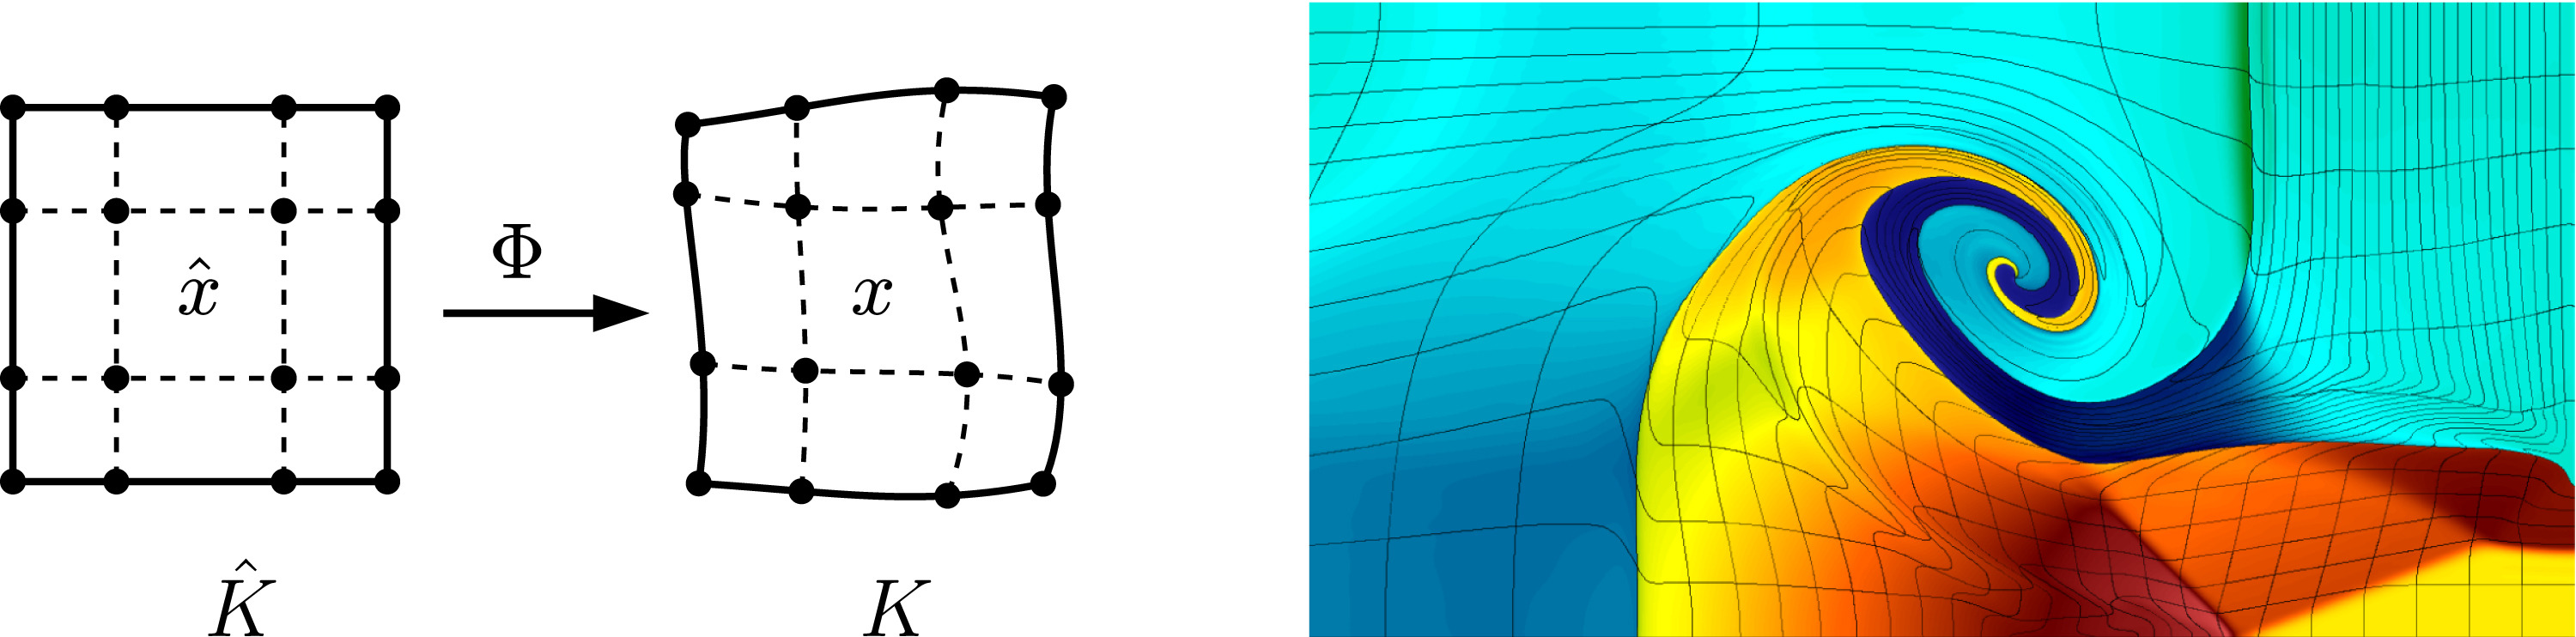
\includegraphics[width=1\linewidth]{image_1.jpg}
\caption{\label{fig:image_1} Left: The mapping $\phi$ from the reference element Kˆ to a bi-cubic element K in physical space with high-order nodes shown as black dots.
Right: Example of a highly deformed high-order mesh from a Lagrangian hydrodynamics simulation}
\end{figure}
\section{Meshes}
This section describes the different types of meshes used in the MFEM library.
\subsection{Conforming Meshes}
Geometric (coordinates) and topological (connectivity) data make up conforming meshes in MFEM. The boundary elements, elements, and vertices make up the topological data. Boundary elements are similar to elements but have one less dimension. Elements have types, attributes, and vertex indices. Richer geometric descriptions are possible by describing the geometric data using either a nodal grid function (nodes) or vertex coordinates. See Figure \ref{fig:image_1} for example
\subsection{Non-Conforming Meshes}
Conforming meshes with restrictions on certain vertices or degrees of freedom are known as non-conforming meshes, or meshes with hanging nodes. By preventing gaps or overlaps in the mesh, these constraints make sure that refined sub-entities stay contained within shared entities. By placing restrictions on nodal grid functions, which represent both unconstrained and constrained degrees of freedom, MFEM manages non-conforming meshes.

\subsection{NURBS Meshes}
NURBS, or Non-Uniform Rational B-Splines, are utilized in discretization and geometric modeling. Because basis functions in NURBS meshes are expressed as tensor products of 1D NURBS basis functions, they resemble high-order polynomial meshes. NURBS meshes are more flexible because the control points, or nodal degrees of freedom, can take part in multiple layers of elements. MFEM uses the Mesh class to represent NURBS meshes; this class contains a nodal grid function that defines NURBS basis functions and control points, as well as a pointer to a NURBSExtension object.
\subsection{Parallel Meshes}
MFEM uses the ParMesh class to support MPI-distributed parallel meshes. ParMesh adds information and capabilities for mesh connections across MPI ranks to the local mesh representation. Every element in the global mesh is a member of a single MPI rank, preventing the ownership or sharing of the same element by multiple processors. GroupTopology objects and processor groups are used to uniformly describe shared entities—such as faces, edges, and vertices—across processors. The required parallel functionality is provided by ParNCMesh and ParNURBSExtension, which are used for parallel non-conforming and NURBS meshes, respectively.

These different mesh types and their representations in MFEM enable users to work with various mesh structures and discretization techniques in parallel computing environments.

\section{Finite Element Discretization}
This section provides an overview of finite element discretization in the context of the MFEM library. It introduces key classes and concepts essential for defining finite element discretization spaces and performing simulations.
\subsection{Finite Elements}
\subsubsection{Reference Element}
A geometric domain defined precisely, including vertices, edges, and faces.
\subsubsection{Map Type}
Describes how a function on the reference element is transformed into a function on a physical element.
\begin{itemize}
        \item VALUE : Used for scalar and vector functions.
        \item INTEGRAL: Also used for scalar and vector functions, preserving integrals.
        \item H\_DIV: Specifically used for vector-valued functions to preserve normal component integrals.
        \item  H\_CURL: Used for vector-valued functions to preserve tangential component integrals.
\end{itemize}
\subsubsection{Degrees of Freedom (DOFs)}
The number of DOFs defines the number of basis functions, associated with specific reference points, used in the finite element space.
\subsection{Finite Element Classes}
Derived from the base class FiniteElement. There are different classes for various types of finite element spaces, including H1, L2, H(curl), and H(div), with different orders.
\subsection{Finite Element Spaces}
\subsubsection{FiniteElementSpace}
Represents a discrete finite element space. It defines the global enumeration of DOFs and is constructed using a mesh and a FiniteElementCollection.
\subsubsection{Vector Dimension}
Represents the number of components in vector spaces.
\subsubsection{Ordering}
Specifies the ordering of vector components in the global DOF enumeration.
\subsection{Discrete de Rham Complex}
Using the de Rham complex, MFEM provides a compatible multi-physics discretization framework that links solution spaces for various PDEs. For kinematic variables, electromagnetic fields, diffusion fluxes, and thermodynamic quantities, it offers finite element spaces.
\subsection{High-Order Spaces}
High-order elements are supported by MFEM, which also offers effective algorithms for managing polynomial order complexity.
\subsection{Input/Output and Visualization}
MFEM can be integrated with a number of tools to visualize fields and meshes. GLVis, VisIt, Netgen, TrueGrid, Gmsh, Exodus, unstructured VTK, and other formats are supported. Additionally, MFEM defines classes for thorough data collection and output, allowing it to work with VisIt and ParaView visualization programs.

This section provides an overview of the main ideas and elements of the MFEM library's finite element discretization, which is necessary for running numerical simulations and performing scientific computing.
\begin{figure*}
\centering
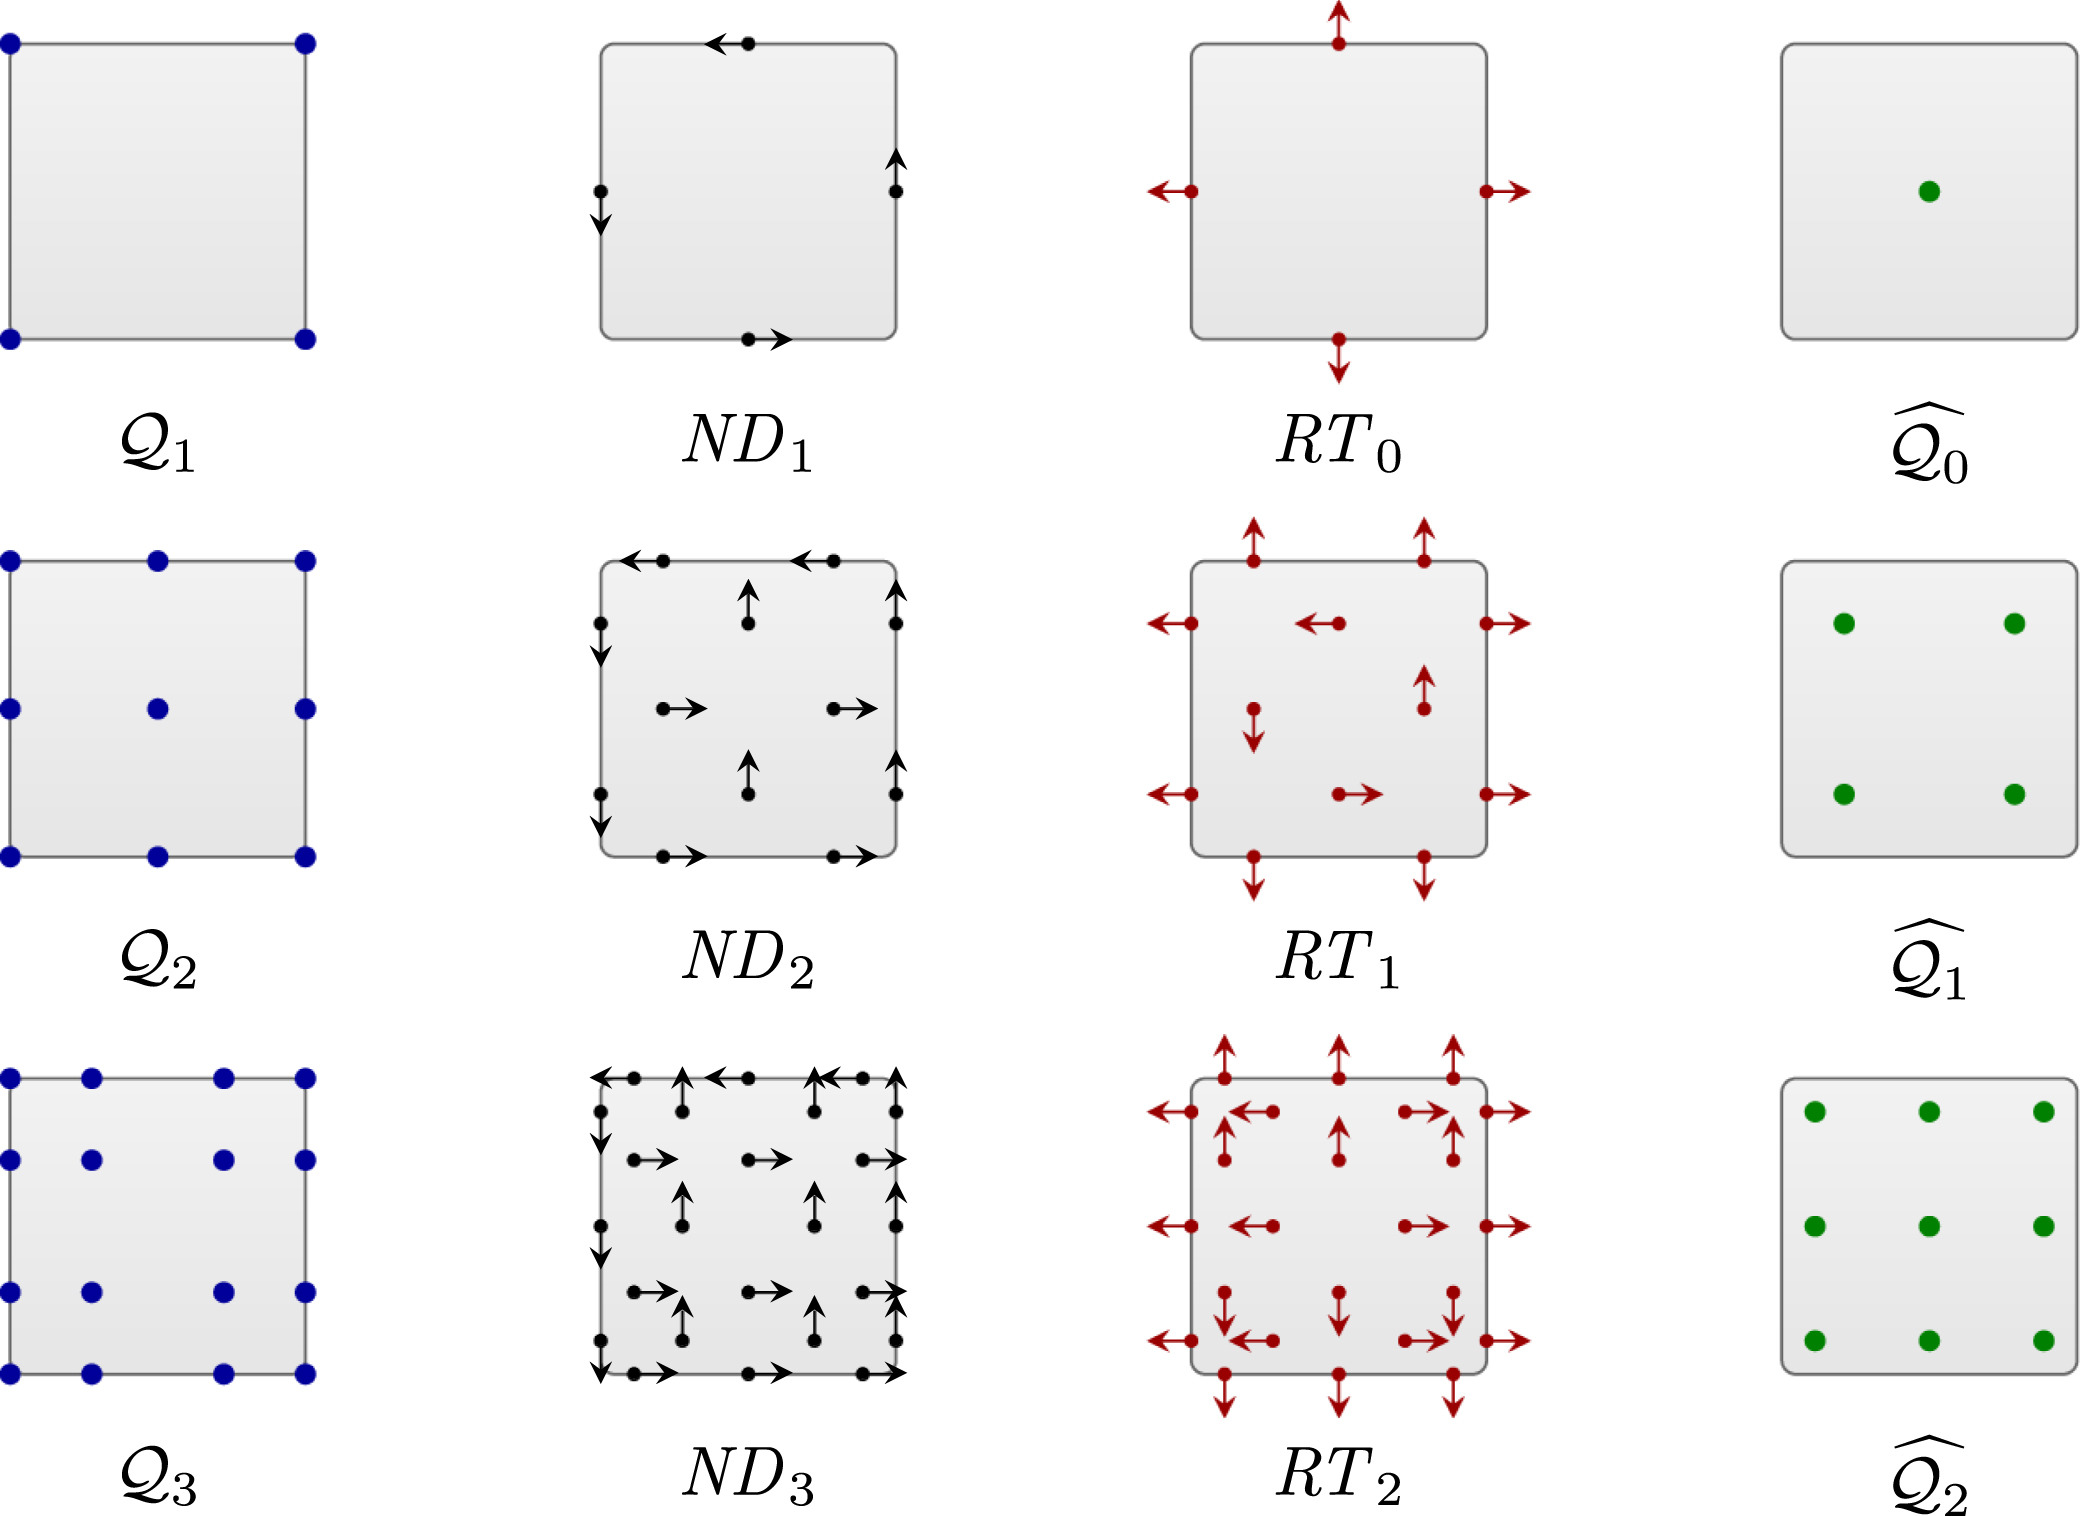
\includegraphics[width=0.4\linewidth]{image_2.jpg}
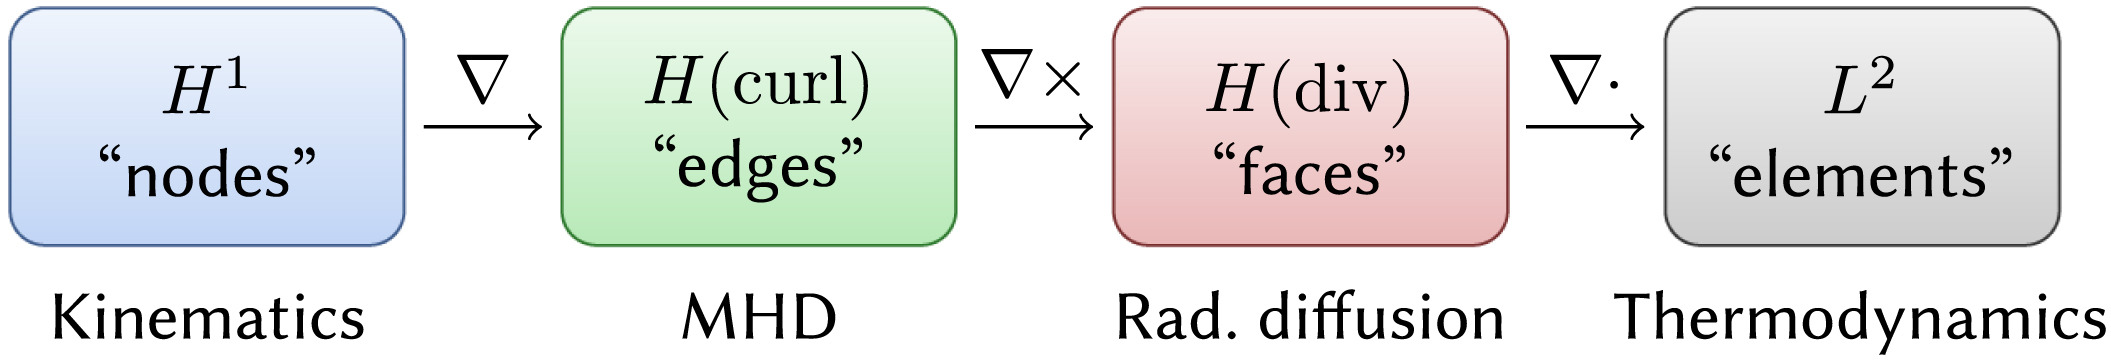
\includegraphics[width=0.5\linewidth]{image_3.jpg}
\caption{\label{fig:image_2} Left: Linear, quadratic and cubic $H^1$ finite elements and their respective H(curl), H(div) and $L^2$ counterparts in 2D.
Right: Example of a highly deformed high-order mesh from a Lagrangian hydrodynamics simulation}
\end{figure*}

\section{ Finite element operators}
\subsection{Discretization Methods}
In order to convert real-world issues governed by partial differential equations into computationally manageable forms, finite element operators are essential. There are several steps in this process, one of which is to change a given linear PDE into a variational form that combines a bilinear form with a linear form.

A flexible library called MFEM offers the fundamental abstractions and building pieces needed to discretize equations. In order to put together the finite element system, users first define two forms: a linear and a bilinear form.

MFEM stands out due to its adaptable integrator system. Integrators are the fundamental components in the PDE that carry out the integrals over the mesh's faces, edges, and elements. They also encapsulate certain mathematical terms. Users can design custom integrators specifically suited to their problems, or they can utilize the many predefined integrators that are available in MFEM.

The MFEM examples provide insightful information about various discretization techniques. For example, you could investigate the use of H1 elements for the Poisson equation or explore more complex methods like discontinuous Petrov-Galerkin (DPG) or discontinuous Galerkin (DG) discretizations. These illustrations highlight the flexibility of the library and aid users in comprehending different finite element methods.

\subsection{Finite Element Linear Systems}
In computational science and engineering, building linear systems from the finite element description of an issue is a basic process. The linear algebra objects in MFEM that are used in this process are Vector and SparseMatrix, both of which have parallel and serial versions.

It is crucial to understand the relationship between linear algebra objects (Vector and SparseMatrix) and finite element objects (GridFunction, LinearForm, and BilinearForm). Users can work with and manipulate both linear algebra structures and finite element representations with ease thanks to this link.

A crucial component of finite element calculations are boundary conditions. By providing techniques such as FormLinearSystem, which prepares linear algebra objects and manages boundary conditions, MFEM makes the application of boundary conditions easier while maintaining the non-singularity of the linear system.

Additionally, more sophisticated methods like hybridization and static condensation are supported by MFEM, allowing for an effective reduction in the size of the linear system.

\subsection{Operator Decomposition}
For effective implementation, it is essential to comprehend the hierarchical structure of finite element operators. Global degrees of freedom are the starting point of the decomposition, which is followed by transitions to subdomains (groups of elements), computations for individual elements, quadrature points in the reference space, and finally back to global degrees of freedom.

MPI parallelism, unstructured mesh topology, finite element basis functions, geometry, and point-wise physics are all divided into different categories within this hierarchical structure. The parallelization and optimization of computations involving finite elements are made easier by this division.

This decomposition revolves around the ideas of operator at quadrature points (D), basis evaluator (B), subdomain restriction (P), and element restriction (G). These constituents function as the fundamental units for the effective assessment of finite element operators.

\subsection{High-Order Partial Assembly}
Reevaluating the entire matrix is a common requirement of high-order finite element methods, which increases computational complexity and memory usage. Sum factorization and partial assembly provide answers to these problems.

It is not necessary to explicitly store the entire matrix when partial assembly is used. Rather, it concentrates on instantaneously applying the operator and evaluating it at each element's quadrature points. Because of its substantial memory requirements and computational complexity reduction, this method works well with high-order finite element methods.

A crucial method in partial assembly is sum factorization, especially for tensor-product element meshes (hexahedra and quadrilaterals). It divides the computations into smaller, easier-to-manage parts, enabling the effective application of operators. High-order discretizations benefit from increased scalability and performance as a result.

\subsection{Parallelization and Challenges}

Parallelization is naturally enabled by the hierarchical structure of finite element operators. For instance, operators can be used to independently apply each element in parallel, making the most of CPUs or GPUs with multiple cores.

Partial assembly parallelization combined with sum factorization makes it possible to efficiently transfer computational workloads to co-processors, like GPUs. Finite element simulations may accelerate significantly as a result of this.

Ensuring data consistency and maintaining synchronization between parallel processes are challenges associated with parallelization. Effective parallel execution of finite element simulations depends on controlling communication and preventing race situations.


In conclusion, libraries such as MFEM offer a rich ecosystem for discretizing PDEs, building linear systems, optimizing computational efficiency, and utilizing parallelism for high-performance computing. Finite element operators are fundamental to many numerical simulations. These ideas are essential for resolving many practical science and engineering issues.

\section{High-performance computing}
This passage discusses various aspects of high-performance computing in the context of the MFEM library.
\subsection{MFEM's Parallelism Handling}
With the help of the Message Passing Interface (MPI) library, MFEM can handle large-scale parallelism effectively. With this method, developers can make use of their current codebase and gain access to parallel processing power by extending serial classes with parallel logic. It is possible to easily add the "Par" prefix to finite element variables and convert serial applications into highly scalable parallel versions by subclassing serial classes. This conversion guarantees that developers can easily switch between serial and parallel versions by streamlining the migration process.

Essentially, MFEM divides the problem domain, also called the mesh, into several segments, each segment being assigned to a distinct MPI task. This partitioning technique guarantees that every processor functions as locally as possible, minimizing the need for excessive inter-processor communication. The parallel mesh object, ParMesh, efficiently expands a regular serial Mesh on each MPI task by adding extra information about shared geometric entities among processors. This enables MFEM to handle distributed data structures effectively.

ParFiniteElementSpace, the parallel equivalent of serial finite element space, also extends it. It describes shared degrees of freedom grouped into communication clusters and spans a regular serial FiniteElementSpace on each task. A number of operations depend on the parallel finite element space, including the provision of the prolongation matrix P for adaptive mesh refinement and parallel assembly.

\subsection{Parallel Assembly and MPI Optimization}
When it comes to parallel assembly, MFEM employs a very effective method. At the local vector (L-vector) level, the finite element stiffness matrix (AL) can be assembled with minimal parallel communication by using K diagonal blocks. By employing asynchronous MPI calls, this method effectively overlaps computation and communication while minimizing MPI messages. The design of MFEM must prioritize reducing communication overhead in order to guarantee high-performance parallel computing.

The PtALP triple matrix product is used by MFEM to achieve the final parallel assembly. This is accomplished using either PETSc routines or the hypre library, which contains the RAP triple-product kernel for algebraic multigrid solvers. The option is determined by the underlying operator type, which is set using the ParBilinearForm class's SetOperatorType method. Users can choose the best algebraic library for their particular problem thanks to MFEM's flexibility in supporting multiple libraries.

\subsection{Scalable Linear Solvers}
A variety of scalable linear solvers are available to users through MFEM. The hypre library's ParCSR format allows for the direct computation and storage of parallel matrices, giving rise to high-performance parallel linear algebra algorithms. Applications can now take advantage of algebraic multigrid preconditioners for improved scalability, even on extremely large parallel tasks, thanks to this integration with Hypre. By using straightforward code, users can apply these scalable preconditioners to solve linear systems with ease, as the examples provided show.
\subsection{GPU Acceleration and Performance Portability}
High-performance computing requires hardware accelerators like GPUs to be supported by MFEM. Applications can choose different backends at runtime and benefit from heterogeneous architectures thanks to it. This guarantees that different hardware configurations and libraries can be utilized according to particular needs and hardware accessibility.

Moreover, the performance portability approach of MFEM is not restricted to any particular framework. Rather, it accommodates several backends with varying features and technological configurations. Optimizing MFEM's performance for different architectures requires this flexibility. To meet the requirements of challenging multi-physics problems, it also offers interoperability with external libraries and software components like hypre, PETSc, and SUNDIALS.

\subsection{Memory Management}
A key element of MFEM's GPU support is memory management. Memory can be allocated and dealt with easily thanks to the Memory class, which serves as a front-end for the internal memory manager. By facilitating effective data transfer between the CPU and GPU, this class maximizes data access and reduces data transfer overhead. It provides read-only, write-only, and read-write access modes to facilitate smooth data transfer and reshape pointers into tensors for easy multi-dimensional indexing within computational kernels.
\subsection{Transition to GPUs and Current Limitations}
Converting current applications to GPUs can be a pretty simple procedure. To make GPU acceleration available, users can configure a device object and turn on partial assembly mode. Code transformation for GPU execution is facilitated by the Memory class and the MFEM\_FORALL macros.

It's crucial to remember that not all integrators have been ported to GPUs as of yet, and MFEM does not support full assembly on GPUs. However, there is a strong commitment to addressing these limitations through active development, with the goal of releasing these features soon.
\subsection{Performance Results}
Initial performance results show the benefits of GPU acceleration over multi-core CPUs, with notable improvements in performance. The findings demonstrate how actively GPU support is developing, with future work aimed at boosting efficiency and broadening MFEM's capabilities.

In conclusion, MFEM's all-encompassing approach to high-performance computing consists of effective parallelism handling, optimized parallel assembly, scalable linear solvers, GPU acceleration, memory management, and ongoing improvements to produce excellent performance results for a variety of applications and hardware setups.

\section{Finite element adaptivity}
Finite element adaptivity is fully supported by MFEM in both serial and parallel settings, including a range of mesh refinement and mesh optimization methods. To achieve precise and effective simulations on high-order unstructured meshes, these abilities are essential. Important facets of MFEM's support for adaptivity comprise:

\subsection{Conforming Adaptive Mesh Refinement (h-Adaptivity)} For tetrahedral meshes, MFEM uses a bisection-based process that facilitates both uniform and local refinement. It is also feasible to refine individual elements locally while forcing neighboring elements to refine as well in order to guarantee a mesh that conforms. Face refinement is handled consistently and effectively by MFEM, which manages consistent refinement across processors in parallel.
\subsection{Non-Conforming Adaptive Mesh Refinement (h-Adaptivity)}
MFEM allows for irregular or non-conforming refinements by extending adaptivity to hexahedral and quadrilateral meshes. This method can handle high-order curved meshes and accept finite element spaces of different degrees. By putting restrictions on degrees of freedom, the technique enables adaptive refinement to continue even in the case of non-conforming elements.

\subsection{Mesh Optimization (r-Adaptivity)}
Target-Matrix Optimization Paradigm (TMOP)-based MFEM offers a framework for optimizing high-order curved meshes. With this method, users can guarantee ideal global mesh attributes, including size, shape, and alignment with particular features, while also managing the quality of the local mesh. Reducing computational resources and enhancing simulation quality depend heavily on mesh optimization.
\subsection{Parallelism}
When utilizing adaptivity strategies on distributed memory systems, MFEM provides robust support for parallel adaptivity, guaranteeing effective communication and load balancing.

\subsection{Extension}
MFEM is a flexible platform for different requirements related to adaptivity and optimization since it enables users to specify unique quality metrics and target construction techniques.

These adaptivity features allow high-resolution and efficient computations on high-order unstructured meshes, enabling users to customize their simulations to the particular requirements of their applications. Furthermore, the continuous development work of MFEM aims to improve simulation performance and accuracy by augmenting adaptivity capabilities and offering additional support for simulation-driven adaptivity.

\section{Applications}


    \begin{table}[H]
        \centering
        \scalebox{1.2}{
        \renewcommand{\arraystretch}{2}
        \begin{tabular}{m{2cm}|m{5cm}m{5cm}}
        \hline
        App. Type & Related Abstract Problems  & Solid Problems\\
        \hline
        \hline
        Examples and Miniapps & Element Discretization of PDE's, Solving Laplace and Poisson Problems, dynamic adaptive mesh refinement & Solving linear and nonlinear elasticity, problems from Maxwell's equations\\
        Electro magnetics & Solving for boundary conditions and source terms in electrostatics. Modeling for Joule heating in electrical conductors. & Solving for boundary conditions and source terms in magnetostatics and time domain electromagnetic wave propagation. \\
        Compressible hydrodynamics & It uses continuous finite element spaces for position and velocity fields and discontinuous spaces for energy fields & modeling compressible inviscid gas dynamics using Euler equations\\
        \end{tabular}}
        \caption{Applications Regarding MFEM}
        \label{tab:First_Table}
    \end{table}

\section{Conclusion}
This article represents a short explanation of the MFEM library which itself is an immerse field. Some of the methods for FEM analysis is covered in a short manner and the mathematical relations are kept plain for ease. All the figures and information here belongs to the authors in the reference section.

\bibliographystyle{plain}
\bibliography{bibliography.bib}
\end{document}